\documentclass[10pt,landscape,a4paper]{article}
\usepackage[utf8]{inputenc}
\usepackage[ngerman]{babel}
\usepackage[T1]{fontenc}
%\usepackage[LY1,T1]{fontenc}
%\usepackage{frutigernext}
%\usepackage[lf,minionint]{MinionPro}
\usepackage{tikz}
\usetikzlibrary{shapes,positioning,arrows,fit,calc,graphs,graphs.standard}
\usepackage[nosf]{kpfonts}
\usepackage[t1]{sourcesanspro}
\usepackage{multicol}
\usepackage{wrapfig}
\usepackage[top=0mm,bottom=1mm,left=0mm,right=1mm]{geometry}
\usepackage[framemethod=tikz]{mdframed}
\usepackage{microtype}
\usepackage{pdfpages}

\let\bar\overline

\newcommand\rd{\mathrm{d}}
\newcommand\om{\omega}
\newcommand\roc{\text{ROC}}

\definecolor{myblue}{cmyk}{0,0,0,1}

\def\firstcircle{(0,0) circle (1.5cm)}
\def\secondcircle{(0:2cm) circle (1.5cm)}

\colorlet{circle edge}{myblue}
\colorlet{circle area}{myblue!5}

\tikzset{filled/.style={fill=circle area, draw=circle edge, thick},
    outline/.style={draw=circle edge, thick}}
    
\pgfdeclarelayer{background}
\pgfsetlayers{background,main}

\everymath\expandafter{\the\everymath \color{myblue}}
\everydisplay\expandafter{\the\everydisplay \color{myblue}}

\renewcommand{\baselinestretch}{.8}
\pagestyle{empty}

\global\mdfdefinestyle{header}{%
linecolor=gray,linewidth=1pt,%
leftmargin=0mm,rightmargin=0mm,skipbelow=0mm,skipabove=0mm,
}

\newcommand{\header}{
\begin{mdframed}[style=header]
\footnotesize
\sffamily
Someone, Signals and Systems\\
Have Fun!
\end{mdframed}
}

\makeatletter % Author: https://tex.stackexchange.com/questions/218587/how-to-set-one-header-for-each-page-using-multicols
\renewcommand{\section}{\@startsection{section}{1}{0mm}%
                                {.2ex}%
                                {.2ex}%x
                                {\color{myblue}\sffamily\small\bfseries}}
\renewcommand{\subsection}{\@startsection{subsection}{1}{0mm}%
                                {.2ex}%
                                {.2ex}%x
                                {\sffamily\bfseries}}



\def\multi@column@out{%
   \ifnum\outputpenalty <-\@M
   \speci@ls \else
   \ifvoid\colbreak@box\else
     \mult@info\@ne{Re-adding forced
               break(s) for splitting}%
     \setbox\@cclv\vbox{%
        \unvbox\colbreak@box
        \penalty-\@Mv\unvbox\@cclv}%
   \fi
   \splittopskip\topskip
   \splitmaxdepth\maxdepth
   \dimen@\@colroom
   \divide\skip\footins\col@number
   \ifvoid\footins \else
      \leave@mult@footins
   \fi
   \let\ifshr@kingsaved\ifshr@king
   \ifvbox \@kludgeins
     \advance \dimen@ -\ht\@kludgeins
     \ifdim \wd\@kludgeins>\z@
        \shr@nkingtrue
     \fi
   \fi
   \process@cols\mult@gfirstbox{%
%%%%% START CHANGE
\ifnum\count@=\numexpr\mult@rightbox+2\relax
          \setbox\count@\vsplit\@cclv to \dimexpr \dimen@-1cm\relax
\setbox\count@\vbox to \dimen@{\vbox to 1cm{\header}\unvbox\count@\vss}%
\else
      \setbox\count@\vsplit\@cclv to \dimen@
\fi
%%%%% END CHANGE
            \set@keptmarks
            \setbox\count@
                 \vbox to\dimen@
                  {\unvbox\count@
                   \remove@discardable@items
                   \ifshr@nking\vfill\fi}%
           }%
   \setbox\mult@rightbox
       \vsplit\@cclv to\dimen@
   \set@keptmarks
   \setbox\mult@rightbox\vbox to\dimen@
          {\unvbox\mult@rightbox
           \remove@discardable@items
           \ifshr@nking\vfill\fi}%
   \let\ifshr@king\ifshr@kingsaved
   \ifvoid\@cclv \else
       \unvbox\@cclv
       \ifnum\outputpenalty=\@M
       \else
          \penalty\outputpenalty
       \fi
       \ifvoid\footins\else
         \PackageWarning{multicol}%
          {I moved some lines to
           the next page.\MessageBreak
           Footnotes on page
           \thepage\space might be wrong}%
       \fi
       \ifnum \c@tracingmulticols>\thr@@
                    \hrule\allowbreak \fi
   \fi
   \ifx\@empty\kept@firstmark
      \let\firstmark\kept@topmark
      \let\botmark\kept@topmark
   \else
      \let\firstmark\kept@firstmark
      \let\botmark\kept@botmark
   \fi
   \let\topmark\kept@topmark
   \mult@info\tw@
        {Use kept top mark:\MessageBreak
          \meaning\kept@topmark
         \MessageBreak
         Use kept first mark:\MessageBreak
          \meaning\kept@firstmark
        \MessageBreak
         Use kept bot mark:\MessageBreak
          \meaning\kept@botmark
        \MessageBreak
         Produce first mark:\MessageBreak
          \meaning\firstmark
        \MessageBreak
        Produce bot mark:\MessageBreak
          \meaning\botmark
         \@gobbletwo}%
   \setbox\@cclv\vbox{\unvbox\partial@page
                      \page@sofar}%
   \@makecol\@outputpage
     \global\let\kept@topmark\botmark
     \global\let\kept@firstmark\@empty
     \global\let\kept@botmark\@empty
     \mult@info\tw@
        {(Re)Init top mark:\MessageBreak
         \meaning\kept@topmark
         \@gobbletwo}%
   \global\@colroom\@colht
   \global \@mparbottom \z@
   \process@deferreds
   \@whilesw\if@fcolmade\fi{\@outputpage
      \global\@colroom\@colht
      \process@deferreds}%
   \mult@info\@ne
     {Colroom:\MessageBreak
      \the\@colht\space
              after float space removed
              = \the\@colroom \@gobble}%
    \set@mult@vsize \global
  \fi}

\makeatother
\setlength{\parindent}{0pt}
\begin{document}
%\footnotesize
\footnotesize
\begin{multicols*}{5}
\section{Modulation}

\subsection*{Sinusoidal Amplitude Modulation}
Synchronous Demodulation: 

$y(t)=cos(\om_c t)x(t)$

$c'(t)=cos(\om_c t + \Delta \om t + \phi)$ (local carrier)

$x_r(t)=x(t)cos(\Delta \om t + \phi)$

Asynchronous Demodulation: 

$ y(t)=cos(\om_c t)[x(t)+A]  $ ,   $A+x(t)>0$ 

no DC component \to $\eta=\frac{E(x^2(t))}{E(x^2(t))+A^2}<\frac{1}{1+PAPR_x}$

\subsection*{Quadrature Modulation}
$y(t)=x_I(t)cos(\om_c t)-x_Q(t)sin(\om_c t)$

$y(t)cos(\om_c t + \phi) \to LPF(\text{Gain}=2) \to x_I(t)cos(\phi)+x_Q(t)sin(\phi)$

$-y(t)sin(\om_c t) \to LPF \to x_Q(t)$

\subsection*{Single-Sideband Modulation}
$x(t)=x_I(t)$

$H_h(j\om)=\begin{cases} -j,& \om >0 \\ j,& \om<0 \end{cases}$ 

$y_{USB}(t) \to X_Q(j\om)=X(j\om)H_h(j\om)$,   note the $\om_{c0}$ of LPF

$y_{SSB}(t) \to X_Q(j\om)=-X(j\om)H_h(j\om)$

spectrum efficiency: $\text{SSB}=\text{QM}=2 \times \text{AM}$

\subsection*{Pulse-Amplitude Modulated Signals}
$y(t)=\Sigma x(nT)p(t-nT)$,   $p(t)=Sa(\frac{\pi t}{T})+p_1(t)$ 

$P_1(j\om)$ is real, $\om_M=\pm \frac{2\pi}{T}$, even, odd around $\frac{\pi}{T}$(ISI-free)

\subsection*{Frequency Modulation}
$y(t)=cos(\om_c t + \theta_c(t))$

$\frac{\rd \theta_c(t)}{\rd t}=k_f x(t)$,   $x(t)=Acos(\om_m t)$

$m_f=\frac{k_f A}{\om_m}$,   $y(t)=cos(\om_c t + m_f sin(\om_m t))$

NB: $m_f << \frac{\pi}{2}$

$y(t) \approx cos(\om_c t)-m_f (sin(\om_m t))(sin(\om_c t))=cos(\om_c t) + 0.5m_f cos(\om_c t + \om_m t) - 0.5m_f cos(\om_c t - \om_m t)$

WM:

\subsection*{Multiplexing and Multiple Access}










\section{Laplace Transform}

$X(s) = \int_{-\infty}^{\infty} x(t) e^{-st} \rd  t$

Unilateral: $\int_{0-}^{\infty}$

\subsection*{Properties}

\emph{Reduced} rational fraction $X(s) = \frac{N(s)}{D(s)}$ (When $s=\infty$ is zero or pole)
% $\int_{-\infty}^{+\infty} e^{-st} e^{-\alpha t} u(t) \rd t = \frac{1}{a+s}(\Re{s}>-a)\\\int_{-\infty}^{+\infty} e^{-st} (-e^{-\alpha t}) u(-t) \rd t = \frac{1}{a+s}(\Re{s}<-a)$

\subsection*{ROC}

Right sided:$(\sigma \in \roc) \to (\Re{s}>\sigma \subseteq \roc)$

Left sided:$(\sigma \in \roc) \to (\Re{s}<\sigma \subseteq \roc)$

Two sided: $\sigma_1<\Re s<\sigma_2$

Bounded by poles or $\infty$, no poles contained in $\roc$

\subsection*{ILT}

$X(s)=\mathcal F\{x(t)e^{-\sigma t}\}\to x(t)=\frac{1}{2\pi j} \int_{\sigma-j\infty}^{\sigma+j\infty} X(s) e^{st}\rd t \\ = \frac{e^{\sigma t}}{2\pi}\int_{-\infty}^{+\infty} X(\sigma + j\om) e^{j\om t}\rd \om$ (when $\Re s =\sigma$ in $\roc$)

$\mathcal L^{-1}\{s^n\} = u_n(t), all~s$

$\mathcal L^{-1}\{\frac{1}{(s+a)^n}\} = \begin{cases} \frac{-t^{n-1}}{(n-1)!}e^{-at}u(-t), & \Re s <-a\\ \frac{t^{n-1}}{(n-1)!}e^{-at}u(t), & \Re s >-a\end{cases}$

\subsection*{Properties(ROC)}

$X_1(s)=\mathcal L\{ x_1(t)\},\roc=R_1 \\ X_2(s)=\mathcal L\{ x_2(t)\},\roc=R_2$

$aX_1(s) + bX_2(s) = \mathcal L\{ax_1(t) + bx_2(t)\}, \roc\supseteq R_1\cap R_2 $ 
($R_1\cap R_2=\emptyset\to \roc=\emptyset$)

$X_1^*(s^*)=\mathcal L\{x_1^*(t)\}, \roc=R_1$

$e^{-s\tau}X_1(s)=\mathcal L\{x_1(t-\tau)\}, \roc=R_1$

$X_1(s-\tau)=\mathcal L\{x_1(t)e^{\tau t}\}, \roc=R_1+\Re{\tau}$

$\frac{1}{|a|}X_1(\frac s a)=\mathcal L\{x_1(at)\}, \roc=aR_1=\{s|\frac s a \in R_1\}$

$X_1(s)X_2(s)=\mathcal L\{x_1(t) * x_2(t) \}, \roc \supseteq R_1\cap R_2$ (This equality may not hold if $R_1\cap R_2=\emptyset$)

$sX(s)=\mathcal L{x'(t)}, \roc \supseteq R_1, X'(s)=\mathcal L\{-tx(t)\}, \roc = R_1$

$\frac 1 sX(s)=\mathcal L\{\int_{-\infty}^t x(\tau)\rd \tau\}, \roc \supseteq (R\cap (\Re s>0))$

\subsection*{Examples}

$\mathcal L\{cos(\om_0 t) u(t)\} = \frac{s}{s^2+\om_0^2}, \mathcal L\{sin(\om_0 t) u(t)\} = \frac{\om_0}{s^2+\om_0^2}$

\section{z Transform}
$X(z) = \sum_{n=-\infty}^{+\infty} x[n] z^{-n}$, $z=e^s$: $\Re s = \sigma \to |z|=e^{\sigma}$

\subsection*{Examples}

$\mathcal Z\{\cos(\om_0 n) u[n]\}=\frac{1-z^{-1}cos\om_0}{1-2z^{-1}cos\om_0+z^{-2}}$

$\mathcal Z\{\sin(\om_0 n) u[n]\}=\frac{z^{-1}sin\om_0}{1-2z^{-1}cos\om_0+z^{-2}}$


\subsection*{inverse z-Transform}

$x[n]=\frac{1}{2\pi j}\oint X(z)z^{n-1}\rd z$
\section{PID}

\subsection*{Linear Feedback}
Forward $H(s)$, Feedback $G(s)$ ($z$ when discrete).

$Q(s) = \frac{Y(s)}{X(s)} = \frac{H(s)}{1+H(s)G(s)}$

Open loop transfer: $\frac{R(s)}{E(s)} = H(s) G(s)$

Error transfer: $\frac{E(s)}{X(s)} = \frac{1}{1 + H(s) G(s)}$

Inverse system: $Q(s) = \frac{1}{\frac{1}{H(s)} + G(s)} \approx \frac{1}{G(s)}$ (when $|H(s)| \gg 1$)

Compensation: (forward $H(j\om)$, backward $K$ ), $Q(s) \approx \frac 1 K$, (approx irrelevant to $H$)

$\text{Gain} \times \text{BW} \equiv \text{Constant}$

\subsection*{PID Control}

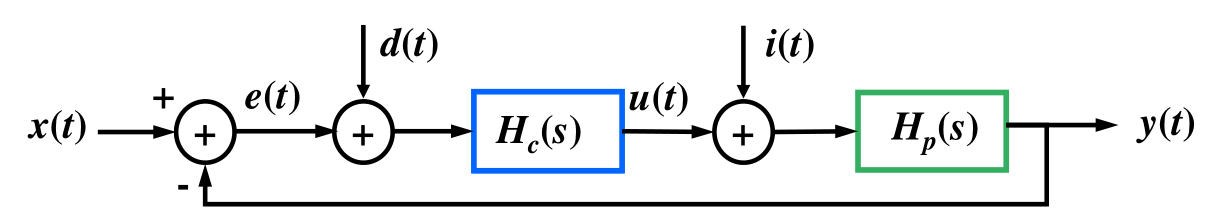
\includegraphics[scale=0.25]{inhalt/pid.png}

$H_o(s) \triangleq H_c(s) H_p(s)$

$E(s) = \frac{X(s)}{1+H_o(s)} - \frac{H_p(s)}{1+H_o(s)} I(s) - \frac{H_o(s)}{1 + H_o(s)} D(s)\\ Y(s) = \frac{H_oX(s)}{1+H_o(s)} + \frac{H_p(s)}{1+H_o(s)} I(s) + \frac{H_o(s)}{1 + H_o(s)} D(s)$

Error transfer:$H_e(s) = \frac{1}{1+H_o(s)}$, close loop: $H(s) = \frac{H_o(s)}{1 + H_o(s)}$, $H(s)+H_e(s) = 1$


\subsubsection*{Steady State Error}
Assume the system to be stable system.

$f(+\infty) = \lim_{s\to 0} sF(s)$

$x(t) = \frac{t^k}{k!} u(t)$, $X(s) = s^{-(k+1)}$

$e_{ss} = \lim_{s\to 0} s E(s) = \lim_{s\to 0} \frac{s^{-k}}{(1 + H_c(s) H_p(s))}$

type-$k$ system: limited non-zero $e_{ss}$ for $k$


$H_p(s) = s^{-m} \hat H_p(s), H_c(s) = s^{-n} \hat H_c(s), 0< |\hat H_p(s)|, |\hat H_c(s)| < \infty $

$e_{ss} = \frac{1}{s^{n+m} + \hat H_p(s)\hat H_c(s)s^{k-(n+m)}} $, type- $m+n$ system for tracking $x$

Similar analysis for interference suppression $I(s)$, type- $n$

\subsubsection*{1.$H_c(s) = k_P$}

$x(t) = u(t)$

$H_p(s) = \frac{A}{s+a}, H(s) = \frac{Ak_p}{s+a+Ak_p}, e_{ss}= \frac{a}{a+k_pA}$

$k_P$ increase $\Rightarrow$ faster response, less error

$H_p(s) = \frac{A}{s^2+a_1s+a_2}, H(s) = \frac{Ak_P}{s^2+a_1s+a_2} = \frac{Ak_P}{Ak_P + a_2} \frac{\om^2}{s^2+2\zeta\om s + \om^2}$ , damped oscillation

$e_{ss} = \frac{a_2}{a_2 + k_PA}$
$k_P$ increase $\Rightarrow$ damp decrease, enhance oscillation, less error

\subsubsection*{2.$H_c(s) =\frac{k_I}{s}$}

$H_p(s) = \frac{A}{s+a}, H(s)=\frac{k_IA}{s^2+as+k_IA}, H_e(s) =\frac{s(s+a)}{s^2+as+k_IA}$ 
$k_I$ increase $\Rightarrow$ damping factor decrease to zero

$x(t)=u(t)\rightarrow e_{ss} = 0, x(t) = tu(t)\rightarrow e_{ss} = \frac{a}{k_IA}$

\subsubsection*{3.$H_c(s) = k_Ds$}

$H_p(s)=\frac{A}{s+a}, H(s)=\frac{k_DAs}{(k_DA+1)s+a}, H(s)=\frac{s+a}{(k_DA+1)s+a}$

$x(t)=u(t), y(\infty)=0$ (can't track constant error)

\subsubsection*{4.$H_c(s) = k_P+k_Ds$}

$H_p(s)=\frac{A}{s+a}, H(s)=\frac{(k_P+k_Ds)A}{(Ak_D+1)s+Ak_P+a}$

$x(t)=u(t), y(\infty)=H(0)=\frac{k_PA}{a+k_PA}, y(0+)=\frac{k_DA}{1+k_DA}$

\subsubsection*{5.$H_c(s) = k_P+\frac{k_I}{s}$ (lower ss error)}

$x(t)=u(t)\rightarrow e(\infty)=0; x(t) = tu(t)\rightarrow e(\infty) = \frac{a}{K_IA}$

\subsubsection*{PLL}


\section{State-Space Analysis}
\subsection*{CT}
$[q_1(t),...,q_L(t)]^T=\boldsymbol{q}(t)$

$\frac{\rd \boldsymbol{q}(t)}{\rd t}=\boldsymbol{Aq}(t)+\boldsymbol{b}x(t)$

$y(t)=\boldsymbol{c^Tq}(t)+dx(t)$

\subsection*{Stability}

for LTI: Asymptotic Stable(about $\lambda_i$)=BIBO

\subsection*{Modal Coordinates(CT for example)}

$[\boldsymbol{v_1},...,\boldsymbol{v_L}]=\boldsymbol{V}$,   $\boldsymbol{A}$'s eigenvectors

$\boldsymbol{q}(t)=\boldsymbol{Vr}(t)$

evolution:  

$\boldsymbol{b}=\boldsymbol{V\beta}$

$\frac{\rd r_i(t)}{\rd t}=\lambda_i r_i(t) + \beta_i x(t)$

output:   

$\boldsymbol{\xi}=\boldsymbol{V^T c}$

$y(t)=\boldsymbol{\xi^Tr}(t)+dx(t)$

\subsection*{Reachability}

$i-\text{th}$ mode is reachable: $\beta_i \neq 0$

Matrix: $\boldsymbol{R_L}=[\boldsymbol{A^{L-1}b}, ..., \boldsymbol{b}]$ is full rank

\subsection*{Observability}

$i-{th}$ mode is observable: $\xi_i \neq 0$

Matrix: $\boldsymbol{O_L}=\begin{bmatrix}c^T\\c^TA\\\ldots\\ c^TA^{L-1}\end{bmatrix}$   L rows
% \input{inhalt/fourier}
% \input{inhalt/filtering}
% \input{inhalt/sampling}
\end{multicols*}
\end{document}